\documentclass[tikz,border=3pt]{standalone}
\usepackage{pgfplots}
\pgfplotsset{compat=1.18}
\usetikzlibrary{arrows.meta,positioning,calc}
\begin{document}
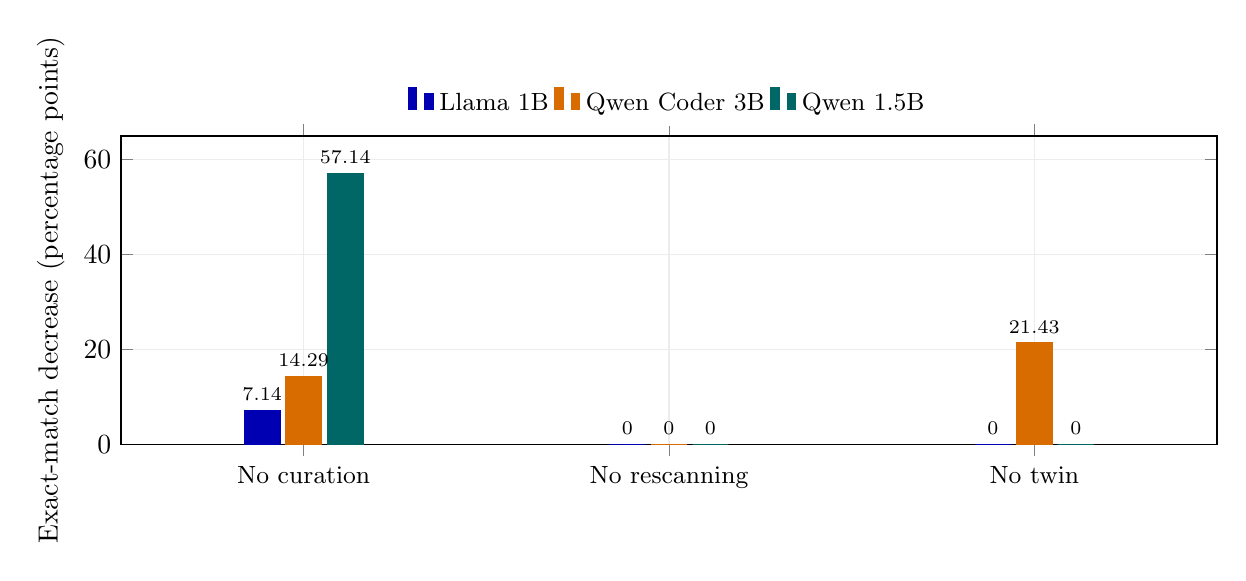
\begin{tikzpicture}
\begin{axis}[width=15.5cm,height=5.5cm,ybar,bar width=13pt,ymin=0,ymax=65,
ylabel={Exact-match decrease (percentage points)},symbolic x coords={No curation,No rescanning,No twin},xtick=data,
grid=major,grid style={gray!15},legend style={font=\small,draw=none,at={(0.5,1.03)},anchor=south,legend columns=3},
xticklabel style={font=\small},nodes near coords,nodes near coords style={font=\scriptsize},enlarge x limits=0.25]
\addplot[fill=blue!70!black,draw=blue!70!black] coordinates {(No curation,7.143) (No rescanning,0.000) (No twin,0.000)};
\addplot[fill=orange!85!black,draw=orange!85!black] coordinates {(No curation,14.286) (No rescanning,0.000) (No twin,21.429)};
\addplot[fill=teal!80!black,draw=teal!80!black] coordinates {(No curation,57.143) (No rescanning,0.000) (No twin,0.000)};
\legend{Llama 1B,Qwen Coder 3B,Qwen 1.5B}\end{axis}\end{tikzpicture}\end{document}